
%(BEGIN_QUESTION)
% Copyright 2007, Tony R. Kuphaldt, released under the Creative Commons Attribution License (v 1.0)
% This means you may do almost anything with this work of mine, so long as you give me proper credit

The following illustration shows a portion of water piping from an overhead view, looking down toward the ground (a ``birds-eye'' view).  The pipe itself is completely level (parallel) with the ground, so that all points along the pipe centerline are at the same height:

$$\includegraphics[width=15.5cm]{i02979x01.eps}$$

The inlet pressure gauge shows 50 PSI, and the velocity of the water entering through the 4 inch pipe is known to be 14 feet per second.  Both pressure gauges are fixed at the centerline of the pipe, and are thus at the exact same height.  Calculate the pressure registered at the outlet gauge (on the 16 inch pipe section) in units of PSI, assuming inviscid (frictionless) flow throughout, and a mass density for water of $\rho$ = 1.951 slugs/ft$^{3}$.

\vskip 10pt

\noindent
{\bf Bernoulli's equation:}

$$z_1 \rho g + {v_1^2 \rho \over 2} + P_1 = z_2 \rho g + {v_2^2 \rho \over 2} + P_2$$

\underbar{file i02979}
%(END_QUESTION)





%(BEGIN_ANSWER)

$P_{out}$ = 51.32 PSI

\vskip 10pt

Note: with a pipe diameter ratio of 4:1 (out:in), the exit velocity will be {\it 16 times} slower than the inlet velocity (1:4)$^{2}$ = (1:16).

%(END_ANSWER)





%(BEGIN_NOTES)


%INDEX% Physics, dynamic fluids: Bernoulli's equation

%(END_NOTES)


